\documentclass{beamer}

\usepackage{amsmath,amsfonts,amssymb,bm}
\usepackage{quantikz}
\usepackage{graphicx}
\usepackage{xcolor}
\usepackage{tikz}
\usetikzlibrary{arrows.meta,positioning,calc,decorations.pathmorphing}

\usetheme{Madrid}

\title{HHL as Spectral Filtering}
\subtitle{Quantum Phase Estimation, Green's Functions, and TDHF}
\author{Morten Hjorth-Jensen}
\date{Spring 2026}

\begin{document}

\frame{\titlepage}

%================================================
\section{Motivation}
%================================================

\begin{frame}{Linear Systems in Physics}
Many physics problems reduce to
\[
A x = b.
\]

Examples:
\begin{itemize}
\item discretized Schr\"odinger and diffusion equations,
\item linear response theory,
\item Green's function methods,
\item time-dependent Hartree--Fock (TDHF),
\item random phase approximation (RPA).
\end{itemize}

The HHL algorithm prepares a quantum state proportional to
\[
|x\rangle \propto A^{-1}|b\rangle.
\]
\end{frame}

%------------------------------------------------

\begin{frame}{The Core Spectral Problem}
Suppose
\[
A|u_j\rangle = \lambda_j |u_j\rangle,
\qquad
|b\rangle = \sum_j \beta_j |u_j\rangle.
\]
Then
\[
A^{-1}|b\rangle
=
\sum_j \frac{\beta_j}{\lambda_j}|u_j\rangle.
\]

Thus HHL implements the spectral map
\[
\lambda_j \mapsto \frac{1}{\lambda_j}.
\]

This is why HHL is best viewed as a \emph{spectral inverse-operator algorithm}.
\end{frame}

%================================================
\section{Spectral Picture}
%================================================

\begin{frame}{Spectral Decomposition of the Operator}
Write
\[
A = \sum_j \lambda_j |u_j\rangle\langle u_j|.
\]
Then formally
\[
A^{-1} = \sum_j \frac{1}{\lambda_j}|u_j\rangle\langle u_j|.
\]

Applying the inverse to the source state:
\[
A^{-1}|b\rangle
=
\sum_j \frac{\beta_j}{\lambda_j}|u_j\rangle.
\]

The algorithm must therefore:
\begin{enumerate}
\item identify the spectral components,
\item apply the inverse weight \(1/\lambda_j\),
\item recombine the result into a state.
\end{enumerate}
\end{frame}

%------------------------------------------------

\begin{frame}{Spectral Filter View}
\centering
\begin{tikzpicture}[scale=0.95]
\draw[->] (-4.5,0) -- (4.5,0) node[right] {\(\lambda\)};
\draw[->] (0,-0.2) -- (0,3.2) node[above] {\(f(\lambda)\)};

\draw[thick,blue,domain=-4:-0.45,samples=100] plot (\x,{1/abs(\x)});
\draw[thick,blue,domain=0.45:4,samples=100] plot (\x,{1/abs(\x)});

\draw[dashed] (-1,0) -- (-1,1);
\draw[dashed] (1,0) -- (1,1);
\node at (2.7,2.3) {\(\displaystyle f(\lambda)=\frac{1}{|\lambda|}\)};
\node[below] at (-1,0) {\(-\lambda_0\)};
\node[below] at (1,0) {\(\lambda_0\)};
\end{tikzpicture}

\vspace{0.3cm}
HHL applies a \emph{spectral filter}:
\[
f(\lambda)=\frac{1}{\lambda}.
\]
Modes with small \(|\lambda|\) are enhanced, while large-\(|\lambda|\) modes are suppressed.
\end{frame}

%================================================
\section{Why QPE Appears}
%================================================

\begin{frame}{Why Quantum Phase Estimation is Needed}
In the original HHL algorithm, we must attach eigenvalue information to each eigenvector:
\[
|u_j\rangle |0\rangle
\longrightarrow
|u_j\rangle |\lambda_j\rangle.
\]

This is done by \textbf{quantum phase estimation (QPE)}.

After QPE, the state becomes
\[
\sum_j \beta_j |u_j\rangle |\lambda_j\rangle,
\]
and only then can we implement
\[
\lambda_j \mapsto \frac{1}{\lambda_j}
\]
through a controlled ancilla rotation.
\end{frame}

%================================================
\section{QPE Inside HHL}
%================================================

\begin{frame}{Setup for QPE}
Assume \(A\) is Hermitian and can be exponentiated:
\[
U = e^{iAt}.
\]

If
\[
A|u_j\rangle = \lambda_j |u_j\rangle,
\]
then
\[
U|u_j\rangle = e^{i\lambda_j t}|u_j\rangle.
\]

Thus the eigenvalue problem for \(A\) becomes a phase problem for \(U\):
\[
e^{i\lambda_j t} = e^{2\pi i \phi_j},
\qquad
\phi_j = \frac{\lambda_j t}{2\pi}.
\]
\end{frame}

%------------------------------------------------

\begin{frame}{QPE Registers}
QPE uses:
\begin{itemize}
\item a \emph{system register} holding the eigenvector,
\item a \emph{clock register} of \(m\) qubits for phase readout.
\end{itemize}

Initial state:
\[
|u_j\rangle \otimes |0\rangle^{\otimes m}.
\]

After Hadamards on the clock register:
\[
|u_j\rangle \otimes
\frac{1}{2^{m/2}}
\sum_{k=0}^{2^m-1} |k\rangle.
\]
\end{frame}

%------------------------------------------------

\begin{frame}{Controlled Powers of the Unitary}
Apply controlled powers of \(U\):
\[
U^{2^0}, U^{2^1}, \dots, U^{2^{m-1}}.
\]

Since
\[
U^{2^\ell}|u_j\rangle = e^{2\pi i 2^\ell \phi_j}|u_j\rangle,
\]
the phase information is kicked back onto the control register.

The state becomes
\[
\frac{1}{2^{m/2}}
\sum_{k=0}^{2^m-1}
e^{2\pi i k \phi_j}
|k\rangle |u_j\rangle.
\]
\end{frame}

%------------------------------------------------

\begin{frame}{Inverse Quantum Fourier Transform}
Applying the inverse quantum Fourier transform (QFT\(^{-1}\)) to the clock register gives an estimate of \(\phi_j\), and hence of \(\lambda_j\):
\[
|u_j\rangle |0\rangle^{\otimes m}
\longrightarrow
|u_j\rangle |\widetilde{\lambda_j}\rangle.
\]

Thus, for a superposition
\[
|b\rangle = \sum_j \beta_j |u_j\rangle,
\]
QPE yields
\[
\sum_j \beta_j |u_j\rangle |\widetilde{\lambda_j}\rangle.
\]
\end{frame}

%------------------------------------------------

\begin{frame}{QPE Circuit Block}
\[
\begin{quantikz}[row sep=0.35cm, column sep=0.3cm]
\lstick{$|u_j\rangle$} & \qw & \qw & \qw & \qw & \qw \\
\lstick{$|0\rangle$} & \gate{H} & \ctrl{-1} & \qw & \qw & \qw \\
\lstick{$|0\rangle$} & \gate{H} & \qw & \ctrl{-2} & \qw & \qw \\
\lstick{$|0\rangle$} & \gate{H} & \qw & \qw & \ctrl{-3} & \gate[wires=3]{\text{QFT}^{-1}}
\end{quantikz}
\]

Here the controlled gates are
\[
U,\quad U^2,\quad U^4,\dots
\]
with \(U=e^{iAt}\).
\end{frame}

%------------------------------------------------

\begin{frame}{QPE Logic in Words}
QPE performs three steps:
\begin{enumerate}
\item Create a superposition of time labels in the clock register.
\item Let each branch accumulate a phase \(e^{i\lambda_j t}\).
\item Fourier analyze those phases to recover \(\lambda_j\).
\end{enumerate}

Hence QPE acts as a quantum spectral analyzer.
\end{frame}

%================================================
\section{The Full HHL Circuit}
%================================================

\begin{frame}{High-Level HHL Circuit}
\[
\begin{quantikz}[row sep=0.35cm, column sep=0.42cm]
\lstick{$|b\rangle$} & \qw & \gate[wires=2,style={fill=blue!15,draw=blue}]{\text{QPE}} & \qw & \gate[wires=2,style={fill=yellow!20,draw=orange}]{\text{Controlled } \lambda^{-1}} & \qw & \gate[wires=2,style={fill=blue!15,draw=blue}]{\text{QPE}^{\dagger}} & \qw & \qw \\
\lstick{$|0\rangle^{\otimes m}$} & \qw & & \qw & & \qw & & \qw & \qw \\
\lstick{$|0\rangle_a$} & \qw & \qw & \qw & \gate{R_y(\theta(\lambda))} & \qw & \qw & \meter{} & \qw
\end{quantikz}
\]

\begin{itemize}
\item Blue block: spectral decomposition and recombination.
\item Yellow block: ancilla rotation implementing the inverse eigenvalue weight.
\end{itemize}
\end{frame}

%------------------------------------------------

\begin{frame}{Step 1: Input State}
Prepare
\[
|b\rangle = \sum_j \beta_j |u_j\rangle.
\]

The full initial state is
\[
\sum_j \beta_j |u_j\rangle |0\rangle^{\otimes m}|0\rangle_a.
\]
\end{frame}

%------------------------------------------------

\begin{frame}{Step 2: After QPE}
After QPE:
\[
\sum_j \beta_j |u_j\rangle |0\rangle^{\otimes m}|0\rangle_a
\longrightarrow
\sum_j \beta_j |u_j\rangle |\lambda_j\rangle |0\rangle_a.
\]

This is the stage where the spectral decomposition becomes explicit.
\end{frame}

%------------------------------------------------

\begin{frame}{Step 3: Controlled Rotation}
Choose the ancilla rotation so that
\[
\sin\frac{\theta(\lambda_j)}{2} = \frac{C}{\lambda_j},
\]
for some constant \(C\).

Then
\[
|\lambda_j\rangle |0\rangle_a
\mapsto
|\lambda_j\rangle
\left(
\sqrt{1-\frac{C^2}{\lambda_j^2}}|0\rangle_a
+
\frac{C}{\lambda_j}|1\rangle_a
\right).
\]
\end{frame}

%------------------------------------------------

\begin{frame}{State After Controlled Rotation}
The total state becomes
\[
\sum_j \beta_j |u_j\rangle |\lambda_j\rangle
\left(
\sqrt{1-\frac{C^2}{\lambda_j^2}}|0\rangle_a
+
\frac{C}{\lambda_j}|1\rangle_a
\right).
\]

The inverse eigenvalue weights are now encoded in the ancilla amplitudes.
\end{frame}

%------------------------------------------------

\begin{frame}{Step 4: Inverse QPE}
Apply \( \text{QPE}^{\dagger} \) to uncompute the eigenvalue register:
\[
\sum_j \beta_j |u_j\rangle
\left(
\sqrt{1-\frac{C^2}{\lambda_j^2}}|0\rangle_a
+
\frac{C}{\lambda_j}|1\rangle_a
\right).
\]

Now the eigenvalue register is disentangled, and only the filtered amplitudes remain.
\end{frame}

%------------------------------------------------

\begin{frame}{Step 5: Postselection}
Conditioning on the ancilla outcome \(|1\rangle_a\), the system collapses to
\[
|x\rangle \propto \sum_j \frac{\beta_j}{\lambda_j}|u_j\rangle
= A^{-1}|b\rangle.
\]

This is the desired quantum state solution.
\end{frame}

%================================================
\section{HHL as Spectral Filtering}
%================================================

\begin{frame}{Operator-Function View}
HHL implements
\[
f(A)|b\rangle
\]
with
\[
f(\lambda)=\frac{1}{\lambda}.
\]

More generally, the logic is:
\begin{itemize}
\item diagonalize the operator,
\item transform eigenvalues with a desired function,
\item reconstruct the state.
\end{itemize}

This places HHL in the wider class of quantum spectral transformation methods.
\end{frame}

%------------------------------------------------

\begin{frame}{Comparison with Time Evolution}
Time evolution applies
\[
e^{-iAt} = \sum_j e^{-i\lambda_j t}|u_j\rangle\langle u_j|.
\]
HHL applies
\[
A^{-1} = \sum_j \frac{1}{\lambda_j}|u_j\rangle\langle u_j|.
\]

So:
\begin{itemize}
\item dynamics multiplies modes by phases,
\item HHL multiplies modes by inverse eigenvalues.
\end{itemize}

This is much closer to response theory than to ordinary time evolution.
\end{frame}

%================================================
\section{Green's Functions and Resolvents}
%================================================

\begin{frame}{Resolvent Operator}
In many-body physics, define the resolvent
\[
G(z) = (zI-H)^{-1}.
\]

If
\[
H|u_j\rangle = E_j |u_j\rangle,
\]
then
\[
G(z)=\sum_j \frac{1}{z-E_j}|u_j\rangle\langle u_j|.
\]

This is exactly the same spectral structure as HHL.
\end{frame}

%------------------------------------------------

\begin{frame}{Green's Function Poles}
\centering
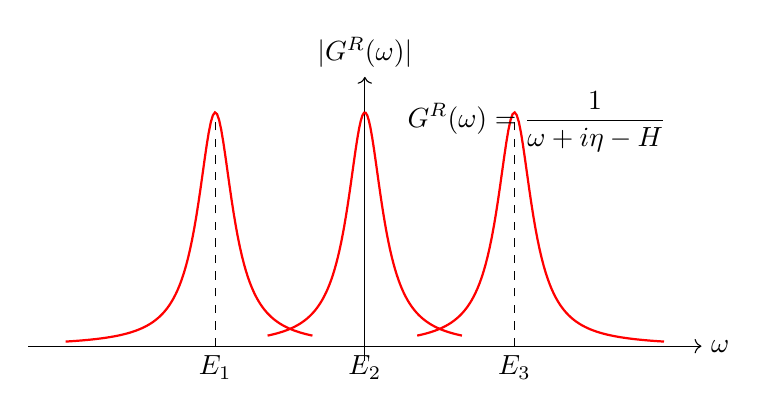
\begin{tikzpicture}[scale=0.95]
\draw[->] (-4.5,0) -- (4.5,0) node[right] {\(\omega\)};
\draw[->] (0,-0.2) -- (0,3.6) node[above] {\(|G^R(\omega)|\)};

\draw[thick,red,domain=-4:-0.7,samples=120] plot (\x,{0.25/((\x+2)^2+0.08)});
\draw[thick,red,domain=-1.3:1.3,samples=120] plot (\x,{0.25/((\x)^2+0.08)});
\draw[thick,red,domain=0.7:4,samples=120] plot (\x,{0.25/((\x-2)^2+0.08)});

\draw[dashed] (-2,0) -- (-2,3.1);
\draw[dashed] (0,0) -- (0,3.1);
\draw[dashed] (2,0) -- (2,3.1);

\node[below] at (-2,0) {\(E_1\)};
\node[below] at (0,0) {\(E_2\)};
\node[below] at (2,0) {\(E_3\)};
\node at (2.3,3.0) {\(\displaystyle G^R(\omega)=\frac{1}{\omega+i\eta-H}\)};
\end{tikzpicture}

\vspace{0.3cm}
The poles of the Green's function correspond to the excitation energies of the system.
\end{frame}

%------------------------------------------------

\begin{frame}{Applying a Green's Function to a Source State}
Let
\[
|b\rangle = \sum_j \beta_j |u_j\rangle.
\]
Then
\[
G(z)|b\rangle
=
\sum_j \frac{\beta_j}{z-E_j}|u_j\rangle.
\]

This has exactly the same structure as
\[
A^{-1}|b\rangle
=
\sum_j \frac{\beta_j}{\lambda_j}|u_j\rangle.
\]

Thus HHL can be interpreted as a quantum Green's-function-style filtering procedure.
\end{frame}

%------------------------------------------------

\begin{frame}{Dynamical Susceptibility}
A standard linear-response object is
\[
\chi(\omega)
=
\langle \psi_0|
\hat{O}^\dagger
\frac{1}{\omega+i\eta-(H-E_0)}
\hat{O}
|\psi_0\rangle.
\]

Defining the source
\[
|b\rangle = \hat{O}|\psi_0\rangle,
\]
we obtain
\[
\chi(\omega)=
\langle b|
\frac{1}{\omega+i\eta-(H-E_0)}
|b\rangle.
\]

Hence HHL is naturally connected to the preparation of response states.
\end{frame}

%================================================
\section{TDHF and Linear Response}
%================================================

\begin{frame}{TDHF Equation}
Time-dependent Hartree--Fock is governed by
\[
i \frac{d\rho}{dt} = [h[\rho],\rho].
\]

Linearizing about a stationary solution,
\[
\rho(t)=\rho_0+\delta\rho(t),
\]
yields a linear equation for the fluctuation \(\delta\rho\).
\end{frame}

%------------------------------------------------

\begin{frame}{Linearized TDHF in Frequency Space}
After Fourier transform, one obtains
\[
(\omega I-\mathcal{L})\,\delta\rho(\omega)=s(\omega),
\]
where
\begin{itemize}
\item \(\mathcal{L}\) is the linearized Liouvillian,
\item \(s(\omega)\) is the driving term.
\end{itemize}

This is exactly of the form
\[
Ax=b.
\]
\end{frame}

%------------------------------------------------

\begin{frame}{TDHF as an Inverse-Operator Problem}
The formal solution is
\[
\delta\rho(\omega)=
(\omega I-\mathcal{L})^{-1}s(\omega).
\]

Thus the TDHF response is a resolvent applied to a source term.

This is precisely the same algebraic structure targeted by HHL.
\end{frame}

%------------------------------------------------

\begin{frame}{TDHF / Linear Response Diagram}
\centering
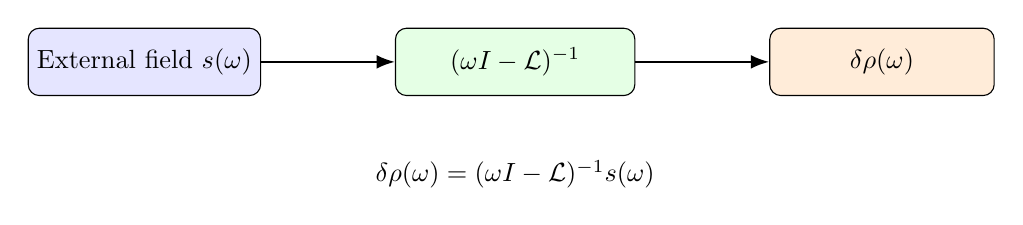
\begin{tikzpicture}[node distance=1.7cm,>=Latex,scale=0.95, every node/.style={scale=0.95}]
\node[draw,rounded corners,fill=blue!10,minimum width=2.8cm,minimum height=0.9cm] (pert) {External field \(s(\omega)\)};
\node[draw,rounded corners,fill=green!10,minimum width=3.2cm,minimum height=0.9cm,right=of pert] (liouv) {\((\omega I-\mathcal{L})^{-1}\)};
\node[draw,rounded corners,fill=orange!15,minimum width=3.0cm,minimum height=0.9cm,right=of liouv] (resp) {\(\delta\rho(\omega)\)};
\draw[->,thick] (pert) -- (liouv);
\draw[->,thick] (liouv) -- (resp);

\node[below=0.7cm of liouv] (text) {\(\delta\rho(\omega)=(\omega I-\mathcal{L})^{-1}s(\omega)\)};
\end{tikzpicture}

\vspace{0.4cm}
The whole linear-response problem is an inverse-operator map from source to response.
\end{frame}

%------------------------------------------------

\begin{frame}{Connection to RPA}
In the small-amplitude limit, TDHF is closely related to the RPA eigenvalue problem
\[
\begin{pmatrix}
A & B \\
-B^* & -A^*
\end{pmatrix}
\begin{pmatrix}
X \\ Y
\end{pmatrix}
=
\omega
\begin{pmatrix}
X \\ Y
\end{pmatrix}.
\]

Equivalently, one can write a driven problem
\[
(\omega I-M)v=s.
\]

Again, the essential structure is resolvent inversion.
\end{frame}

%================================================
\section{Conceptual Picture}
%================================================

\begin{frame}{Physical Role of QPE in HHL}
From a physics viewpoint:
\begin{itemize}
\item QPE performs a spectral decomposition of the operator,
\item the controlled rotation applies a resolvent-like inverse weight,
\item inverse QPE recombines the filtered eigenmodes.
\end{itemize}

So the logic of HHL is
\[
\text{spectral analysis}
\;\rightarrow\;
\text{inverse weighting}
\;\rightarrow\;
\text{state reconstruction}.
\]
\end{frame}

%------------------------------------------------

\begin{frame}{Unified Conceptual Diagram}
\centering
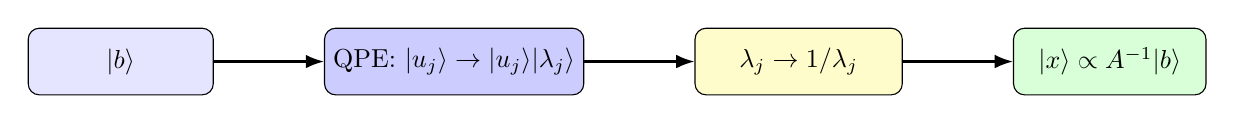
\begin{tikzpicture}[node distance=1.4cm,>=Latex,scale=0.94, every node/.style={scale=0.94}]
\node[draw,rounded corners,fill=blue!10,minimum width=2.5cm,minimum height=0.9cm] (input) {\(|b\rangle\)};
\node[draw,rounded corners,fill=blue!20,minimum width=3.0cm,minimum height=0.9cm,right=of input] (qpe) {QPE: \(|u_j\rangle \to |u_j\rangle|\lambda_j\rangle\)};
\node[draw,rounded corners,fill=yellow!20,minimum width=2.8cm,minimum height=0.9cm,right=of qpe] (filter) {\(\lambda_j \to 1/\lambda_j\)};
\node[draw,rounded corners,fill=green!15,minimum width=2.6cm,minimum height=0.9cm,right=of filter] (output) {\(|x\rangle \propto A^{-1}|b\rangle\)};
\draw[->,thick] (input) -- (qpe);
\draw[->,thick] (qpe) -- (filter);
\draw[->,thick] (filter) -- (output);
\end{tikzpicture}

\vspace{0.5cm}
This is the same logic as in Green's-function and linear-response theory.
\end{frame}

%================================================
\section{Caveats}
%================================================

\begin{frame}{Important Caveats}
The conceptual connection is strong, but practical implementation requires:
\begin{itemize}
\item efficient Hamiltonian simulation or block encoding,
\item well-conditioned matrices,
\item efficient state preparation,
\item care with non-Hermitian response matrices.
\end{itemize}

For non-Hermitian problems one often uses a Hermitian embedding such as
\[
\mathcal{H}=
\begin{pmatrix}
0 & M \\
M^\dagger & 0
\end{pmatrix}.
\]
\end{frame}

%================================================
\section{Summary}
%================================================

\begin{frame}{Summary}
\begin{itemize}
\item In the original HHL algorithm, \textbf{QPE is essential}.
\item QPE is the block that resolves the operator spectrally.
\item HHL then implements the spectral filter
\[
\lambda_j \mapsto \frac{1}{\lambda_j}.
\]
\item This makes HHL naturally connected to
\begin{itemize}
\item resolvents,
\item Green's functions,
\item susceptibilities,
\item TDHF and RPA,
\item frequency-domain linear response.
\end{itemize}
\end{itemize}
\end{frame}

%------------------------------------------------

\begin{frame}{Final Conceptual Equivalence}
\[
\boxed{
A^{-1}|b\rangle
\;\sim\;
(zI-H)^{-1}|b\rangle
\;\sim\;
(\omega I-\mathcal{L})^{-1}s
}
\]

\vspace{0.4cm}
\[
\boxed{
\text{HHL}=
\text{QPE}
+
\text{spectral inversion}
+
\text{state reconstruction}
}
\]

HHL is therefore best interpreted as a quantum inverse-operator method.
\end{frame}

\end{document}
